\documentclass[12pt]{article}

	\usepackage[utf8]{inputenc}
	\usepackage[brazilian]{babel}
	\usepackage{hyperref}
	\usepackage{lipsum}
	\usepackage{geometry}
	\usepackage[skip=5pt plus1pt, indent=20pt]{parskip}
	\usepackage{indentfirst}
	\usepackage{amsthm,amssymb,amsmath}
	\usepackage{minted}
	\usepackage{graphicx}
	
	\geometry{left=3cm, top=3cm, right=2cm, bottom=2cm}
	
	\title{\textbf{Engenharia de Software 2 - Relatório TP1}}
	\author{\textbf{Matheus Flávio Gonçalves Silva - 2020006850}}
	\date{\parbox{\linewidth}{\centering%
    Universidade Federal de Minas Gerais (UFMG)\endgraf
    Belo Horizonte - MG - Brasil\endgraf\bigskip
    \href{mailto:matheusfgs@ufmg.br}{matheusfgs@ufmg.br}}}
	
	\begin{document}

\maketitle

%%%%%%%%%%%%%%%%%%%%%%%%%%%%%%%%%%%%%%%%%%%%%%%%%%%%%%%%%%%%%%%%%%%%%%%%%%%%%%

\section {Membros}
Matheus Flávio Gonçalves Silva


\section{Análise de qualidade com Lizard}
\subsection{Execução da Ferramenta Lizard}
\begin{figure}[h]
	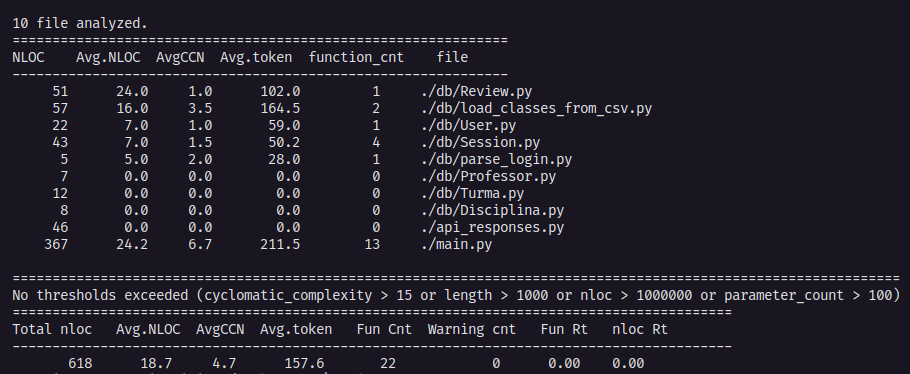
\includegraphics[scale=0.52]{Figure1.png}
	\caption{Saída da execução da ferramenta Lizard no Backend}	
\end{figure}
\par Conforme visto acima, a maioria das funciondalidades estão localizadas no arquivo \textbf{main.py}. Assim sendo, o foco da análise e modificação manter-se-á nas funções presentes nesse arquivo.

\subsection{Análise da Função mais complexa}
\par Ao analisar o código, a função mais complexa é a função \textbf{fetch\_review()}. Esta função está diretamente relacionada com a filtragem e ordenação das reviews de acordo com o semestre, professor, disciplina, classificação, podendo ser dinamicamente alterada de acordo com a preferência do usuário em tempo de uso.
\par Assim sendo, essa função faz uso de consultas ao banco de dados com base nos filtros fornecidos, além de realizar o processamento dos resultados retornados pelo banco e retorna os dados obtidos como resposta ao frontend para exibição correta das reviews. Trata-se da função mais importante do sistema, afinal, de nada adianta fazer uma review a respeito de qualquer coisa que seja e essas reviews não serem exibidas.
\par Dentre as estruturas e paradigmas envolvidos na função, temos a manipulação de listas, a utilização de filtros de pesquisa, além da ordenação dinâmica de acordo com a seleção do usuário.

\section {Adicionais}
\par A partir desse ponto, encontram-se explicações e documentações adicionais que não foram exigidas no PDF segundo o TP. Contudo, por questão de facilidade, foram acrescentadas a partir dessa sessão para maior conforto. Os items 1 e 3 pedidos na especificação encontram-se a seguir.

\newpage

\section {Explicação sobre o sistema}
Para esse sistema web é idealizado um fórum de avaliação a respeito de professores da UFMG com dados referentes ao período de 2020/1 a 2023/1, seleção do semestre lecionado, além da validação se o professor deu aula da matéria especificada no semestre selecionado. Além disso, pode-se selecionar se serão feitas avaliações de forma anônima ou sem anonimato de acordo com a escolha do usuário ao criar a postagem.

\section {Tecnologias}
\begin {itemize}
\item Quart (Backend)
\par Foi escolhido o Quart como backend pela facilidade da manipulação da linguagem Python e pela similaridade com o framework Flask utilizado para desenvolvimento Web. De certo modo, pode-se dizer que o Quart é a reimplementação do Flask com a possibilidade de execução de funções assíncronas.
\item React (Frontend)
\par Foi escolhido o React como ferramenta para desenvolvimento do frontend pela maior intimidade com esse framework.
\item MongoDB (Banco de Dados)
\par Para o banco de dados foi escolhido o MongoDB pela possibilidade de utilização do MongoDB Compass facilitar a correção de pequenos problemas, a visualização dos dados e correção do banco. Foram cogitados também os bandos MySQL e SQLite, mas deixados de lado em virtude da experiência de maior facilidade de lidar com o MongoDB. 
\end {itemize}

\section{Refatoração}

\par 
\newpage
%%%%%%%%%%%%%%%%%%%%%%%%%%%%%%%%%%%%%%%%%%%%%%%%%%%%%%%%%%%%%%%%%%%%%%%%%%%%%%
\section{Questão 4}
\begin{minted}[
    frame=lines,
    framesep=2mm,
    baselinestretch=1.2,
    fontsize=\footnotesize,
    linenos
    ]{python}
função poligonoSimples(arestas)
	eventos = lista vazia
	para cada aresta em arestas
		adicione aresta.ponto_inicial e aresta.ponto_final à lista eventos

	ordene eventos por coordenada x e depois por coordenada y

	segmentos_ativos = árvore balanceada vazia

	para cada evento em eventos
		segmento = evento.segmento
		
		se evento é ponto_inicial do segmento
			insira segmento em segmentos_ativos
			segmento_acima = encontre segmento acima do atual em
			segmentos_ativos

			segmento_abaixo = encontre segmento abaixo do atual em
			segmentos_ativos

			se interseção(segmento, segmento_acima) ou
			interseção(segmento, segmento_abaixo)
			
				retorne falso
				
			senão
				segmento_acima = encontre segmento acima do atual
				em segmentos_ativos
				
				segmento_abaixo = encontre segmento abaixo do atual
				em segmentos_ativos

			se interseção(segmento_acima, segmento_abaixo)
				retorne falso

			remova segmento de segmentos_ativos

	retorne verdadeiro
\end{minted}
\par Este algoritmo verifica se um polígono de n vértices é simples em tempo O(n log n), pois processa todos os eventos em ordem e usa uma estrutura de dados balanceada para armazenar e buscar os segmentos ativos.
\newpage
%%%%%%%%%%%%%%%%%%%%%%%%%%%%%%%%%%%%%%%%%%%%%%%%%%%%%%%%%%%%%%%%%%%%%%%%%%%%%%
\section{Questão 5}
\par Suponha que p e q sejam os dois pontos mais distantes. Além disso, suponha que p está no interior do casco convexo. Em seguida, construa o círculo cujo centro é q e que tem p no círculo. Então, se tivermos algum vértice do casco convexo que esteja fora deste círculo, entre esse vértice e q há uma distância maior do que entre p e q. Então, sabemos que todos os vértices da casca convexa estão dentro do círculo. Isso significa que os lados do casco convexo consistem em segmentos de linha contidos no círculo. Assim, a única maneira que eles poderiam conter p, um ponto no círculo é se fosse um vértice, mas supusemos que p não era um vértice do casco convexo, o que é uma contradição.
%%%%%%%%%%%%%%%%%%%%%%%%%%%%%%%%%%%%%%%%%%%%%%%%%%%%%%%%%%%%%%%%%%%%%%%%%%%%%%%

\section{Questão 6}
\par Será utilizada a triangulação de orelhas:
\begin{minted}[
    frame=lines,
    framesep=2mm,
    baselinestretch=1.2,
    fontsize=\footnotesize,
    linenos
    ]{python}
função triangulaçãoOrelhas(polígono)
	se orientação(polígono) é horário
		inverta a ordem dos vértices de polígono

	vértices_ativos = copie os vértices do polígono para uma nova lista
	triângulos = lista vazia

	enquanto tamanho de vértices_ativos > 3
		para i de 0 até tamanho de vértices_ativos - 1
			a = vértices_ativos[i]
			b = vértices_ativos[(i + 1) % tamanho de vértices_ativos]
			c = vértices_ativos[(i + 2) % tamanho de vértices_ativos]

            se éOrelha(a, b, c, vértices_ativos)
				adicione (a, b, c) à lista triângulos
				remova b de vértices_ativos
				pare o loop
	adicione o último triângulo formado pelos 3 vértices restantes à lista de triângulos
	retorne triângulos

função éOrelha(a, b, c, vértices)
	se ângulo(a, b, c) >= 180 graus
		retorne falso
	triângulo = (a, b, c)
	para cada vértice em vértices
		se vértice não é igual a a, b ou c e vértice está dentro do triângulo
			retorne falso
	retorne verdadeiro
\end{minted}
\end{document}
